%%%%%%%%%%%%%%%%%%%%%%%%%%%%%%%%%%%%%%%%%%%
%                                         %
% This file should only be made of \input %
%                                         %
%%%%%%%%%%%%%%%%%%%%%%%%%%%%%%%%%%%%%%%%%%%

\chapter{Le client}

	\paragraph{}La partie client de notre application sert à interagir avec 
l'utilisateur humain. Basiquement, l'utilisateur tape des commandes et le 
client lui renvoie un résultat calculé par le daemon.
	
	\section{Architecture logique du client}

La figure \ref{client} illustre l'architecture de notre client. Tout d'abord, 
le client se charge de créer une socket permettant de se connecter à son daemon
, avec l'IP et le port adéquat. Il crée ensuite un thread qui s'occupe de gérer
 l'envoi des commandes tapées par l'utilisateur, en exécutant la fonction 
\verb"send_cmd()". Cette fonction crée elle aussi un thread qui, par le biais 
de la fonction \verb"recv_resp()", s'occupe d'afficher à l'écran les réponses 
aux commandes reçues du daemon.

\begin{center}
\begin{figure}[h]
    \centering
    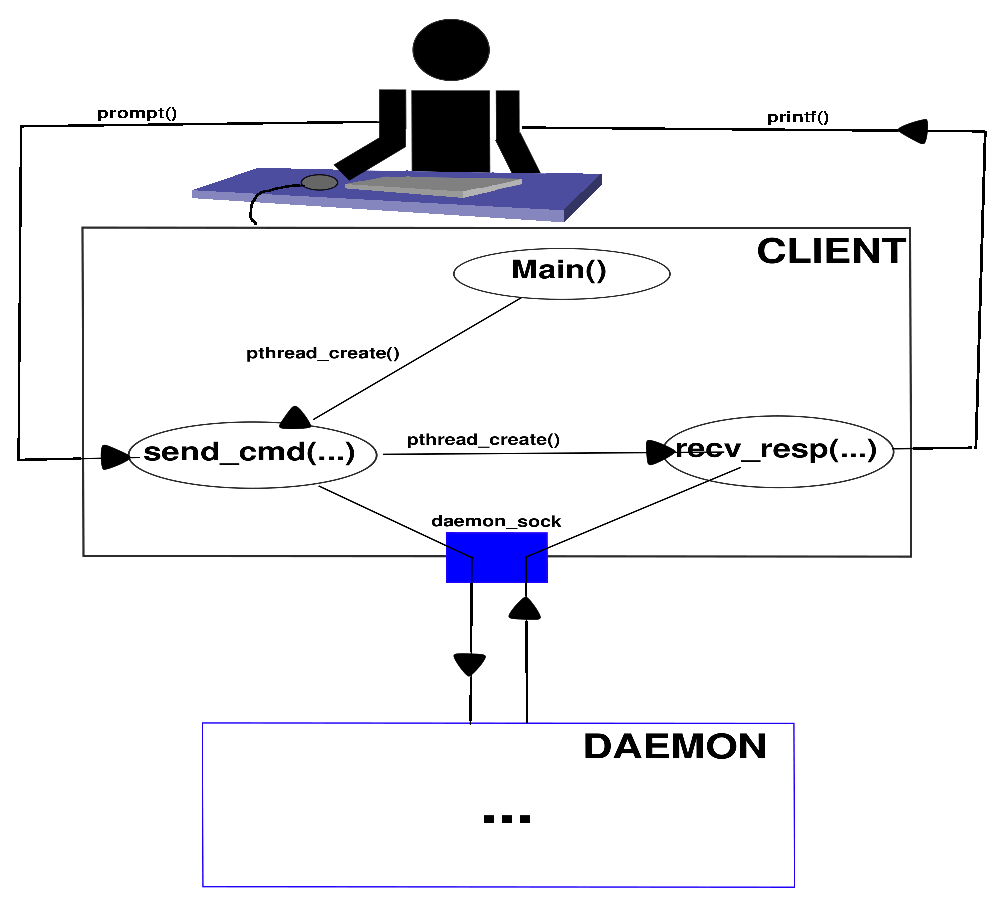
\includegraphics[scale=1.4]{client/archi_client.eps}
    \caption{Architecture du client}
    \label{client}
\end{figure}
\end{center}
	
	\section{Gestion des requ\^etes}

Actuellement, notre client sait gérer les requêtes suivantes :
\begin{itemize}
\item help : affiche une aide
\item list [options] : donne la liste des ressources disponibles sur le réseau 
      sous la forme: \verb"cle nom taille \n"
\item info: affiche des informations/statistiques sur l'état du programme.
\item connect ip:port: indique au programme de se connecter à un autre 
      programme
\item raw ip:port cmd: envoie la commande de protocole cmd à un programme. 
\end{itemize}

D'après la documentation, le client doit être également capable de gérer les 
requêtes suivantes :
\begin{itemize}
\item set : fournit la liste des options disponibles dans le programme
\item set option=valeur: modifie la valeur d'une option
\item get cle: récupère la ressource cle
\item download : affiche des informations sur les fichiers en cours de 
      récupération (format libre)
\item upload : affiche des informations sur les fichiers en cours de transfert
      (format libre)
\end{itemize}
	
	\section{Implémentation actuelle}
	
	\paragraph{}conclusion...
